\documentclass[sans, aspectratio=169]{beamer}
\usepackage{eulervm}
\usepackage[scaled ]{helvet}
\usepackage[utf8]{inputenc}
\usepackage{multimedia}

\usepackage[T1]{fontenc}

\title{\textbf{{\LARGE  Plasma for the space exploration}}\\
On the Hall effect thruster performances}
\date[JS-EDOM2018]{journées scientifiques de l'EDOM - 15/02/2018}
\author[A. Tavant]{Antoine Tavant}

%\usetheme{LPP}
\usepackage{template/beamerthemeLPP}
\begin{document}

\begin{frame}
\titlepage
\end{frame}

\begin{frame} 
	\frametitle{Propulsion for satellites} 
	\framesubtitle{Introduction} 

	\begin{columns}
		\begin{column}{0.75\linewidth}
		
			\begin{itemize} 
				\item Increasing use/need satellite
				\item Propulsion is key : life time, capability, etc. 

			\end{itemize}
			
			\begin{figure}[hbtp]
			%TODO : use 'total satellite instead
				\centering
				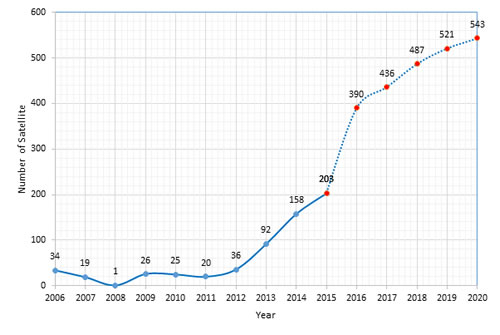
\includegraphics[scale=0.3]{images/sattelite-number.jpg}
				%\caption{•}
			\end{figure}
			
			
							
		\end{column}
		
		\begin{column}{0.3\linewidth}
			\begin{flushright}
			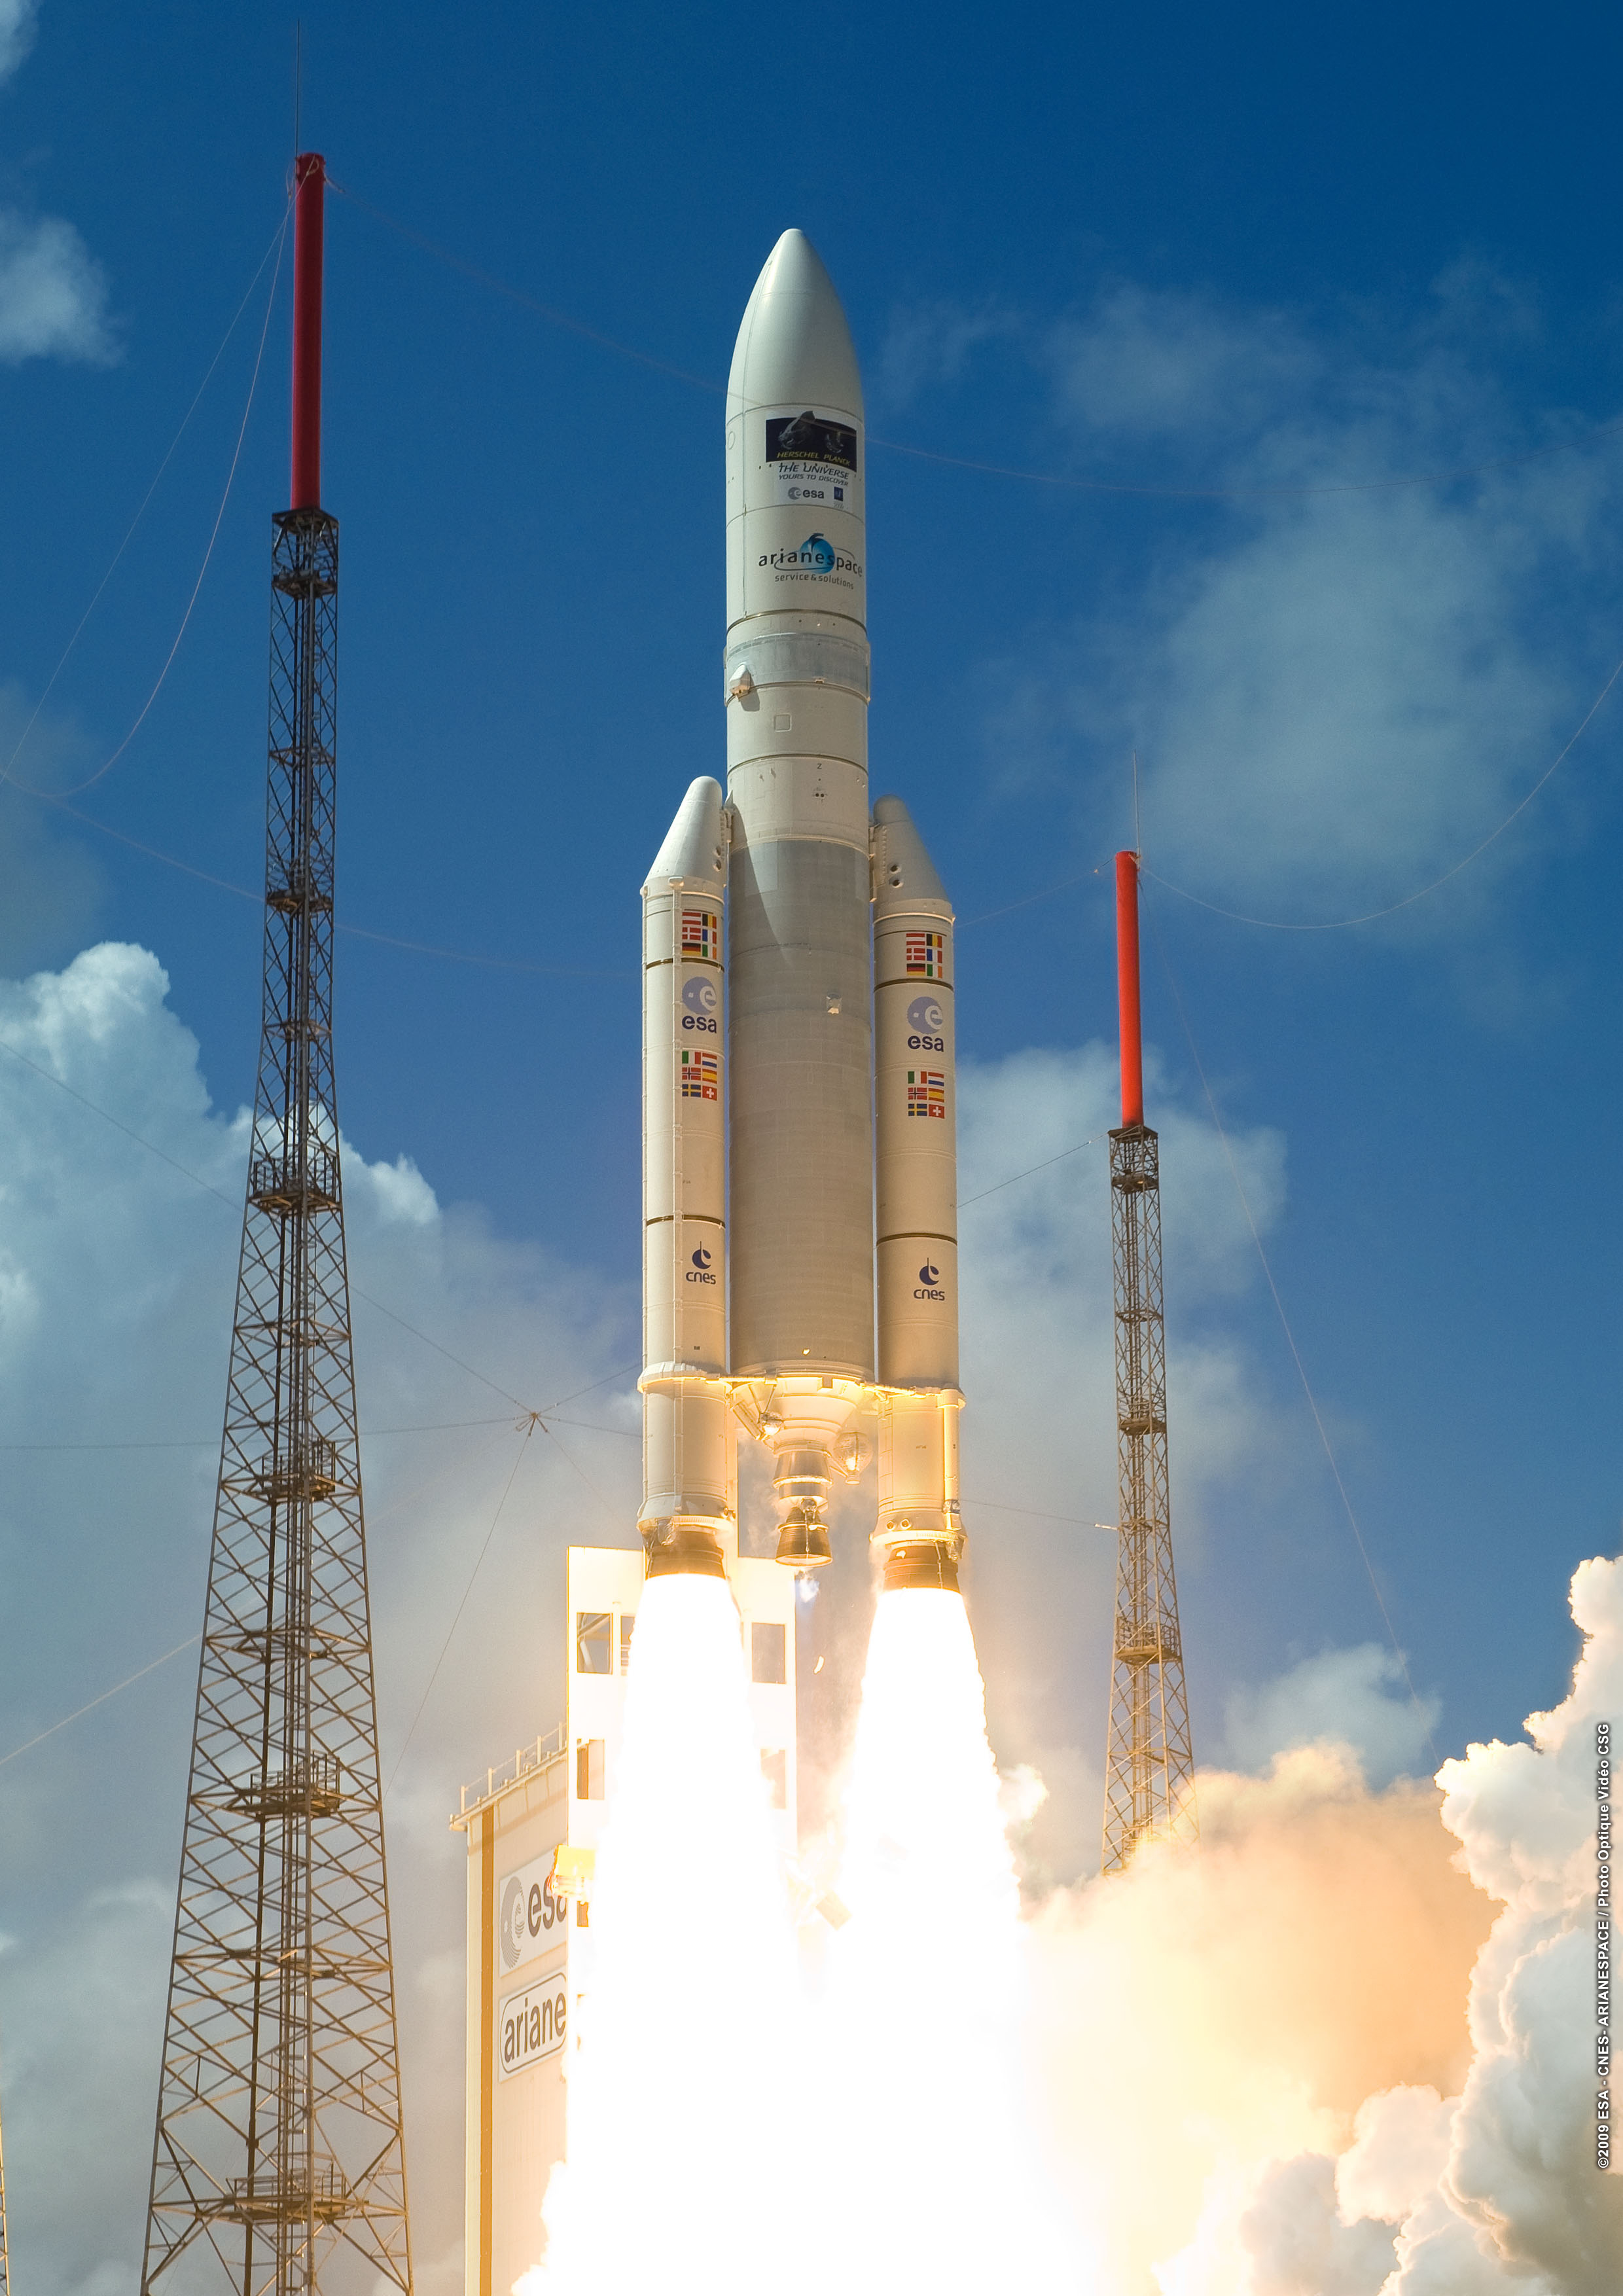
\includegraphics[scale=0.2]{images/arian5.jpg} 
			\end{flushright}
			
		\end{column}
		
	\end{columns}
	
\end{frame}

\begin{frame} 
	\frametitle{The Hall effect Thrusters} 
	\framesubtitle{Introduction} 
	\begin{itemize} 
		\item Space exploration need ever better thrusters to propel spacecraft behong the limits
		\item Hall Effect Thrusters (HET) is a very promissing technology :
		\begin{itemize} 
			\item High exhaust velocity ($\sim 12 km/s$)
			\item Succesfully used since 1970s
			\item \textit{Smart1} spacecraft used it to the moon (ESA, 2009)
		\end{itemize}
	\end{itemize}
	
	%\vspace{0.2cm}
	\renewcommand{\arraystretch}{1.2}% Wider
	\begin{center}
		\begin{tabular}{c|c|c}
			Exhaust velocity & Dry mass & mass at launch \\ \hline 
			$1 km/s$ &   $2 T $     &  $5 T$ \\
			$10 km/s$&  $ 2 T  $   &  $3 T$
		\end{tabular}
	\end{center}
	
	%\vspace{0.2cm}
	However: \textbf{the HET is still poorly understood}

\end{frame}

\begin{frame} 
\frametitle{What don't we know ?} 
\framesubtitle{Introduction} 
Better inderstanding of HET is more and more important. However :

\begin{itemize}
\item Performance (thrust, efficentcy, etc.) isn't predictable yet
	\begin{itemize}
		\item the wall effect is poorly understood
		\item the electron mobility is anormaliously high ($\sim 10 \times$)
	\end{itemize}
\item The life time isn't predictable
	\begin{itemize}
		\item Walls are eroded by ion impact sputtering
		\item Walls resistes from 1000 h to 7000h
		\item Anormalous wall erosion are also observed
	\end{itemize}
\end{itemize}

\textbf{Why ?} Because plasma physics are \textbf{difficult}

\end{frame}

\begin{frame}
	\frametitle{Plasma Beam Instability} 
	\framesubtitle{Some Plasma Physics} 

	An exemple of "simple" plasma behavious : the plasma-beam instability.

\begin{columns}

\begin{column}{0.55\linewidth}
The system is simple:
	\begin{itemize}
		\item a static plasma background
		\item an electron beam with high velocity $v_b >> v_{th}$
		\item Collision are neglected (low pressure)
		\item uniform density
	\end{itemize}
\end{column}

\begin{column}{0.35\linewidth}
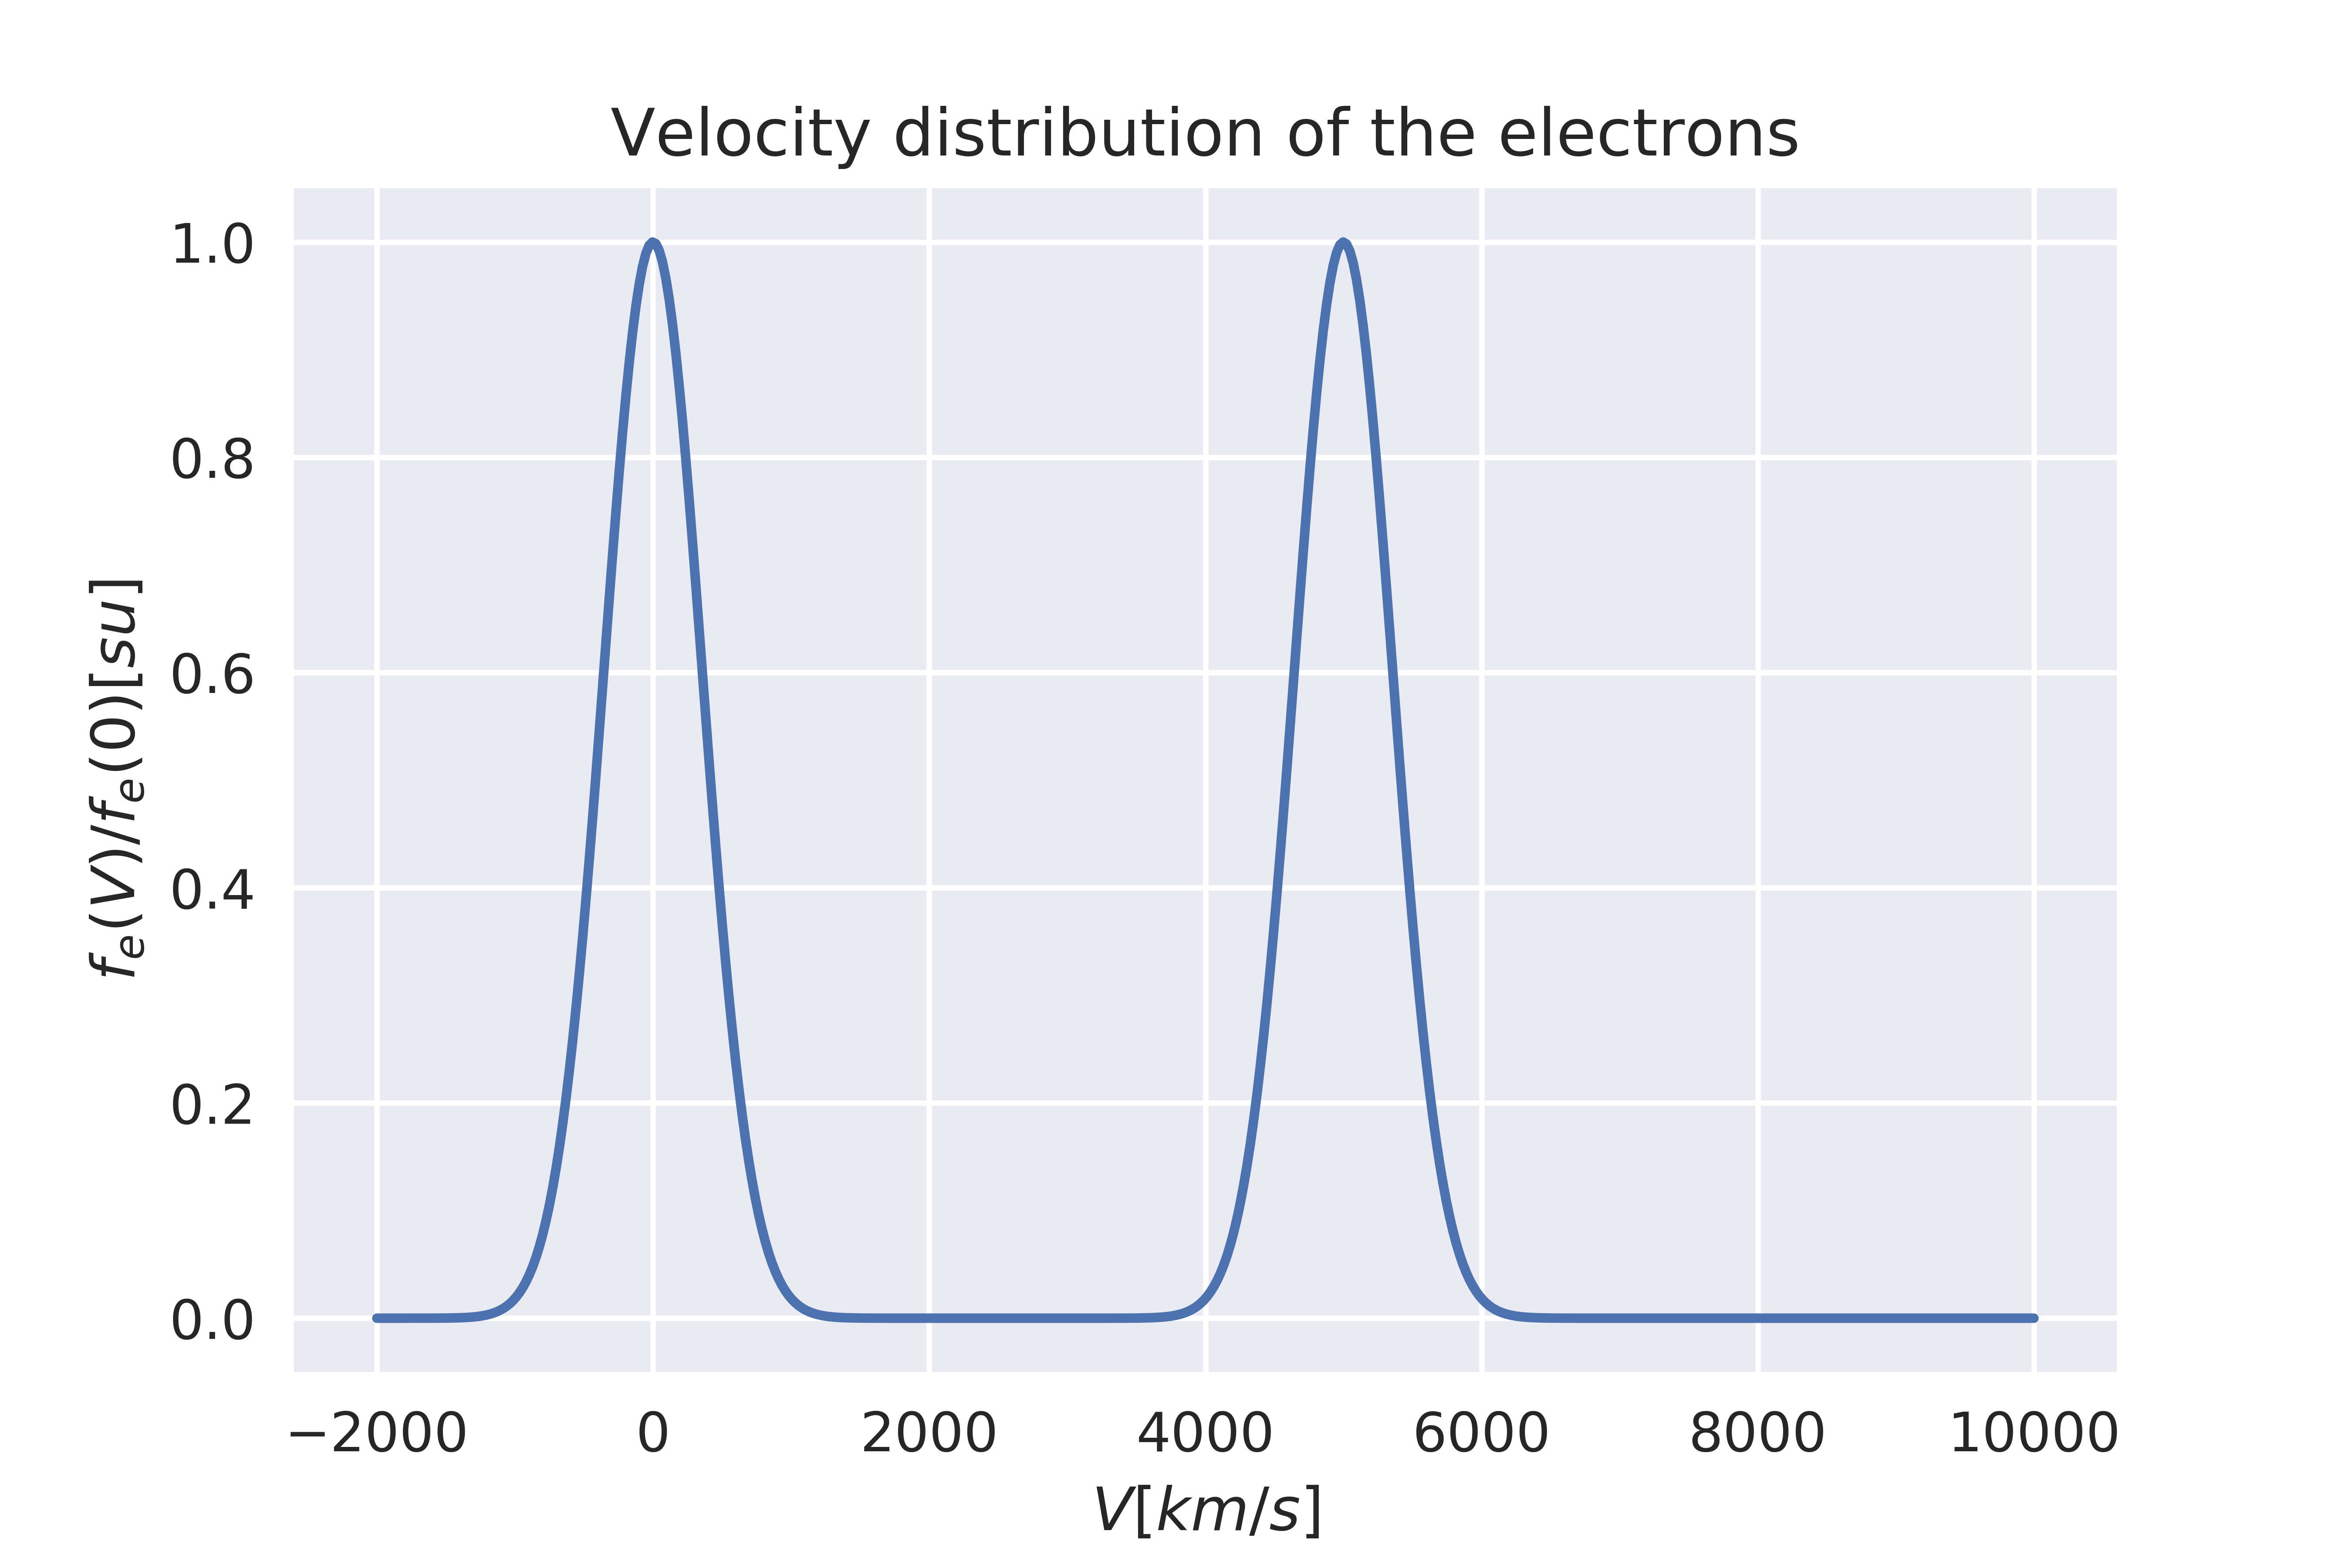
\includegraphics[scale=0.4]{images/plasma_beam_f_v.png} 
\end{column}

\end{columns}	

\end{frame}

\begin{frame}
	\frametitle{Plasma Beam Instability} 
	\framesubtitle{Some Plasma Physics} 

	An exemple of "simple" plasma behavious : the plasma-beam instability.

\begin{columns}

\begin{column}{0.55\linewidth}
The system is simple:
	\begin{itemize}
		\item a static plasma background
		\item an electron beam with high velocity $v_b >> v_{th}$
		\item Collision are neglected (low pressure)
		\item uniform density
		
	\end{itemize}
\end{column}

\begin{column}{0.35\linewidth}
	\movie[width=5cm,height=4cm,poster,showcontrols=true]{}{images/BeamInstability.mp4}
\end{column}

\end{columns}	

\end{frame}


\begin{frame} 
	\frametitle{Hall Effect Thruster : presentation} 
	\framesubtitle{More details} 

\begin{columns}

	\begin{column}{0.45\linewidth}
		\begin{figure}[hbtp]
		\centering
		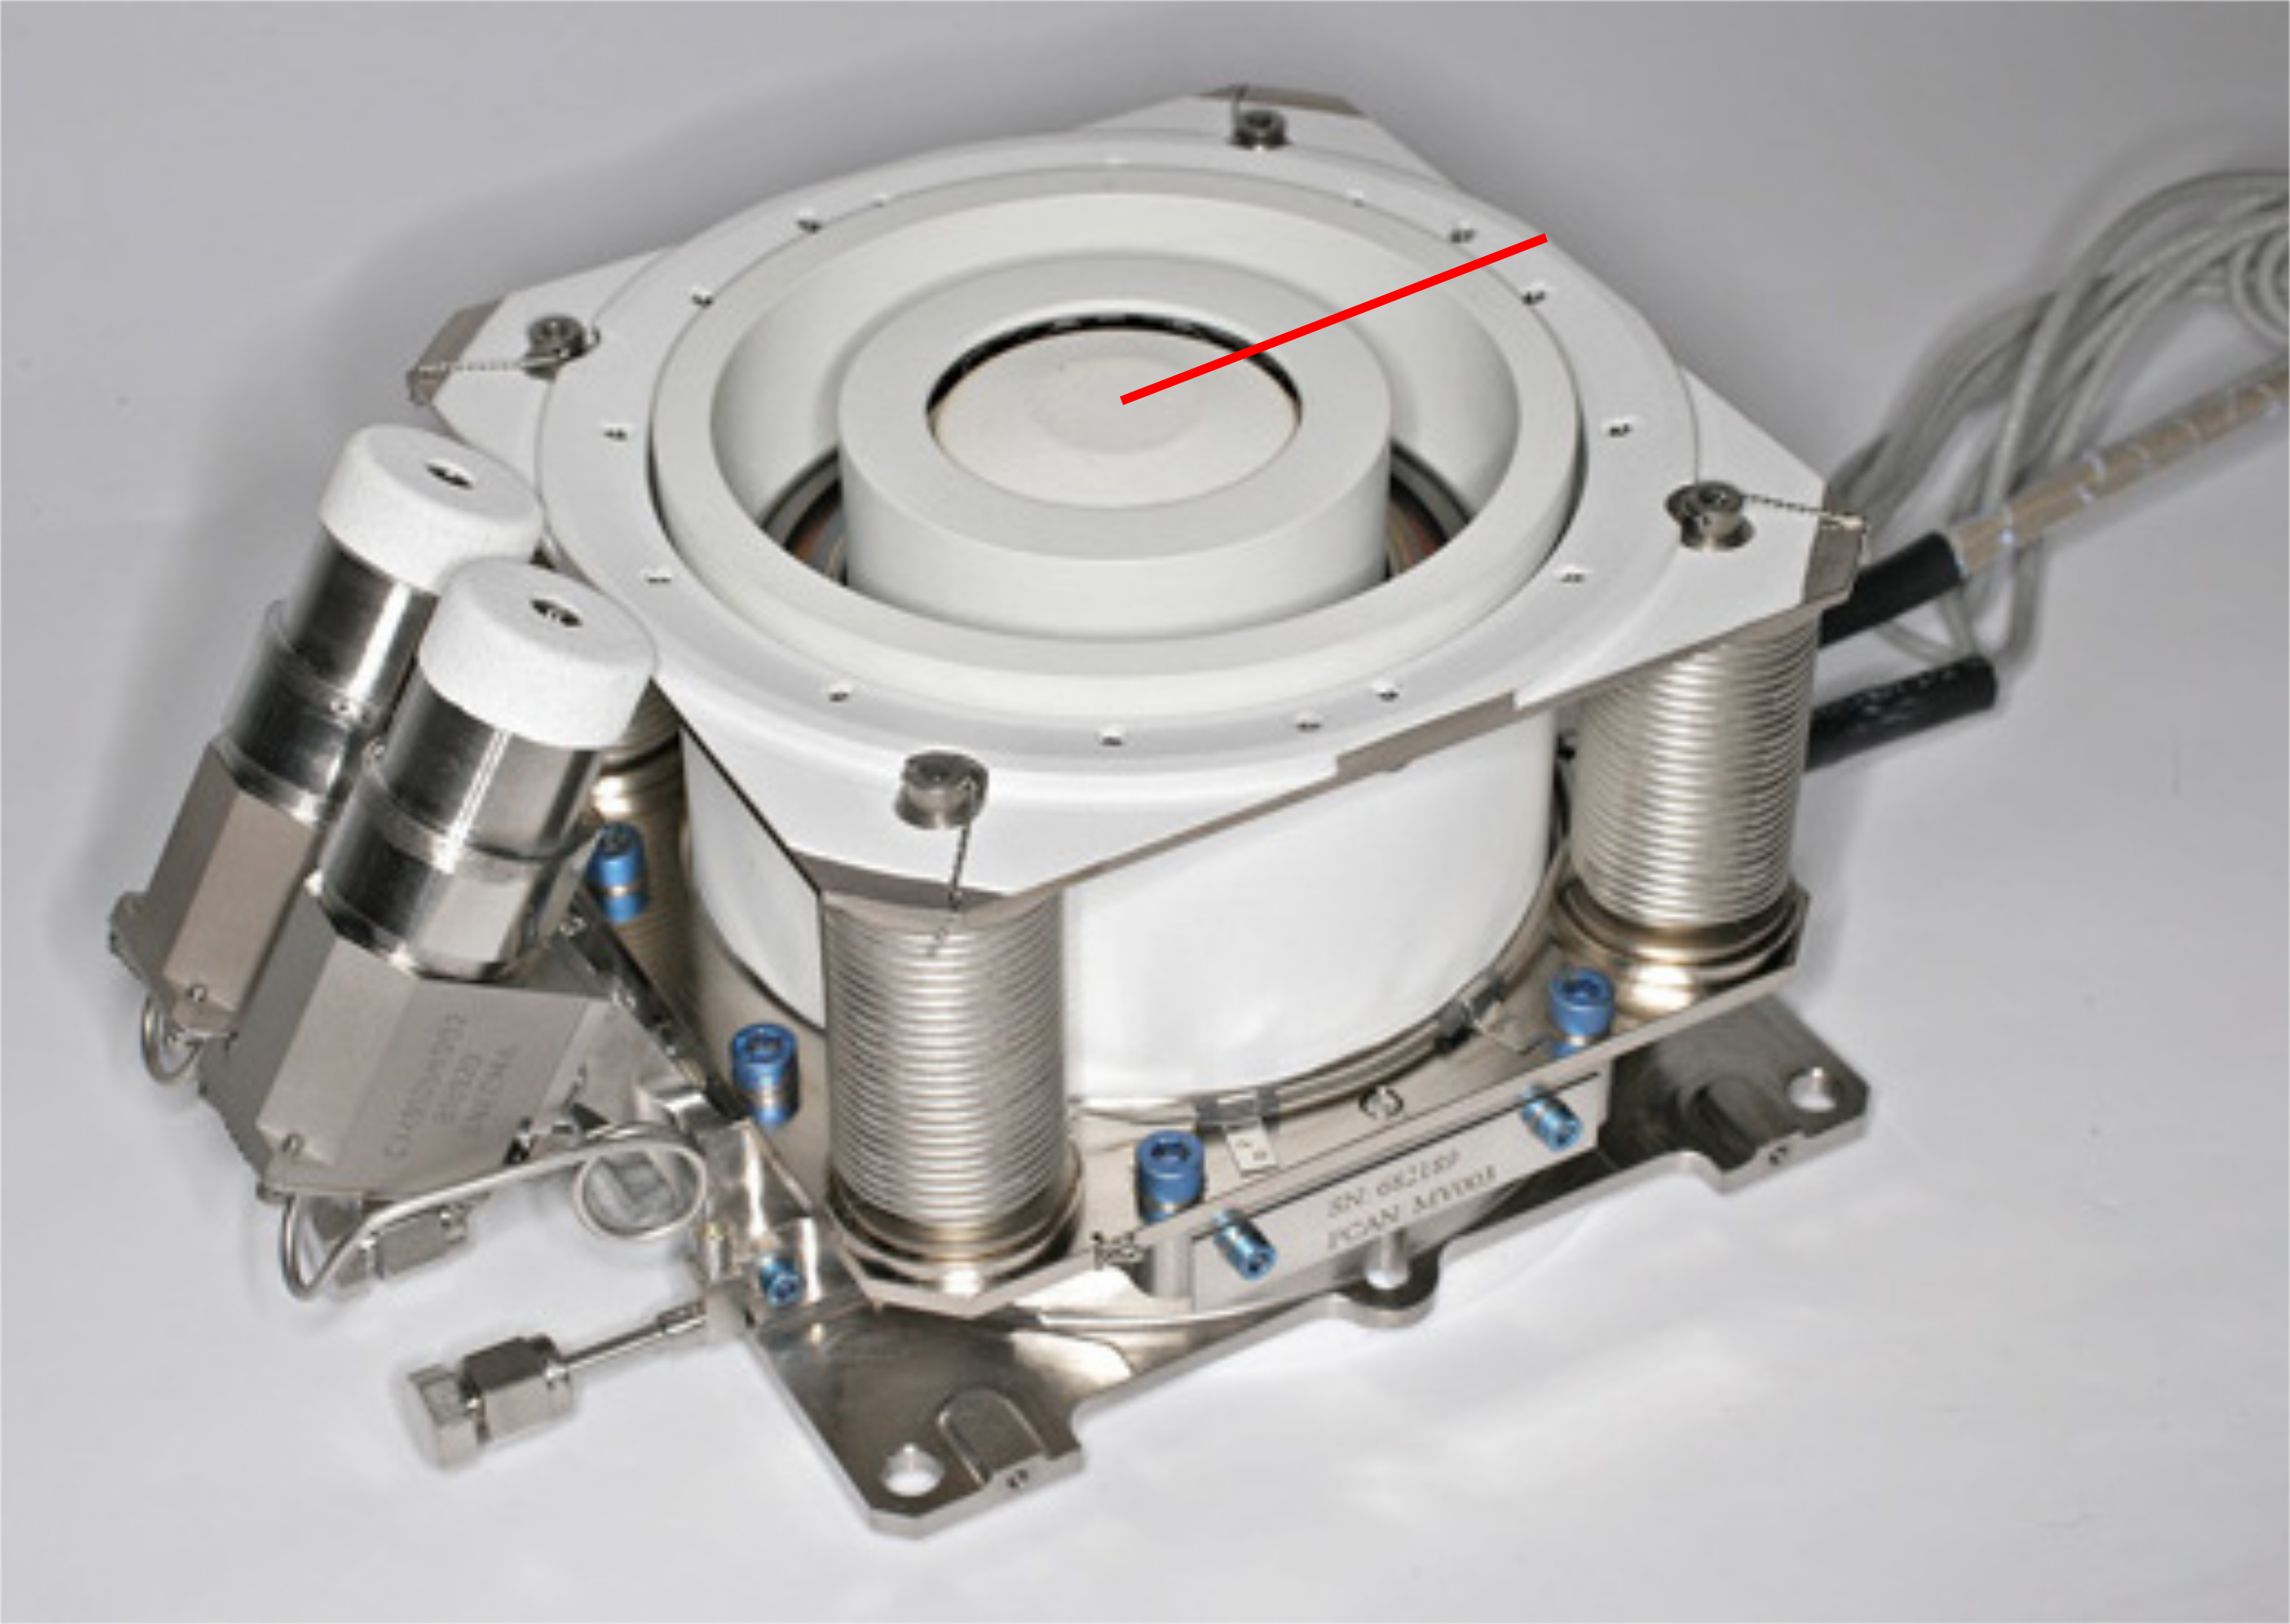
\includegraphics[scale=0.25]{images/PPS1350-G.png}
		\caption{Hall Effect Thruster (PPS-1350, Safran )}
		\end{figure}
	
	\end{column}

	\begin{column}{0.45\linewidth}
		\begin{figure}[hbtp]
		\centering
		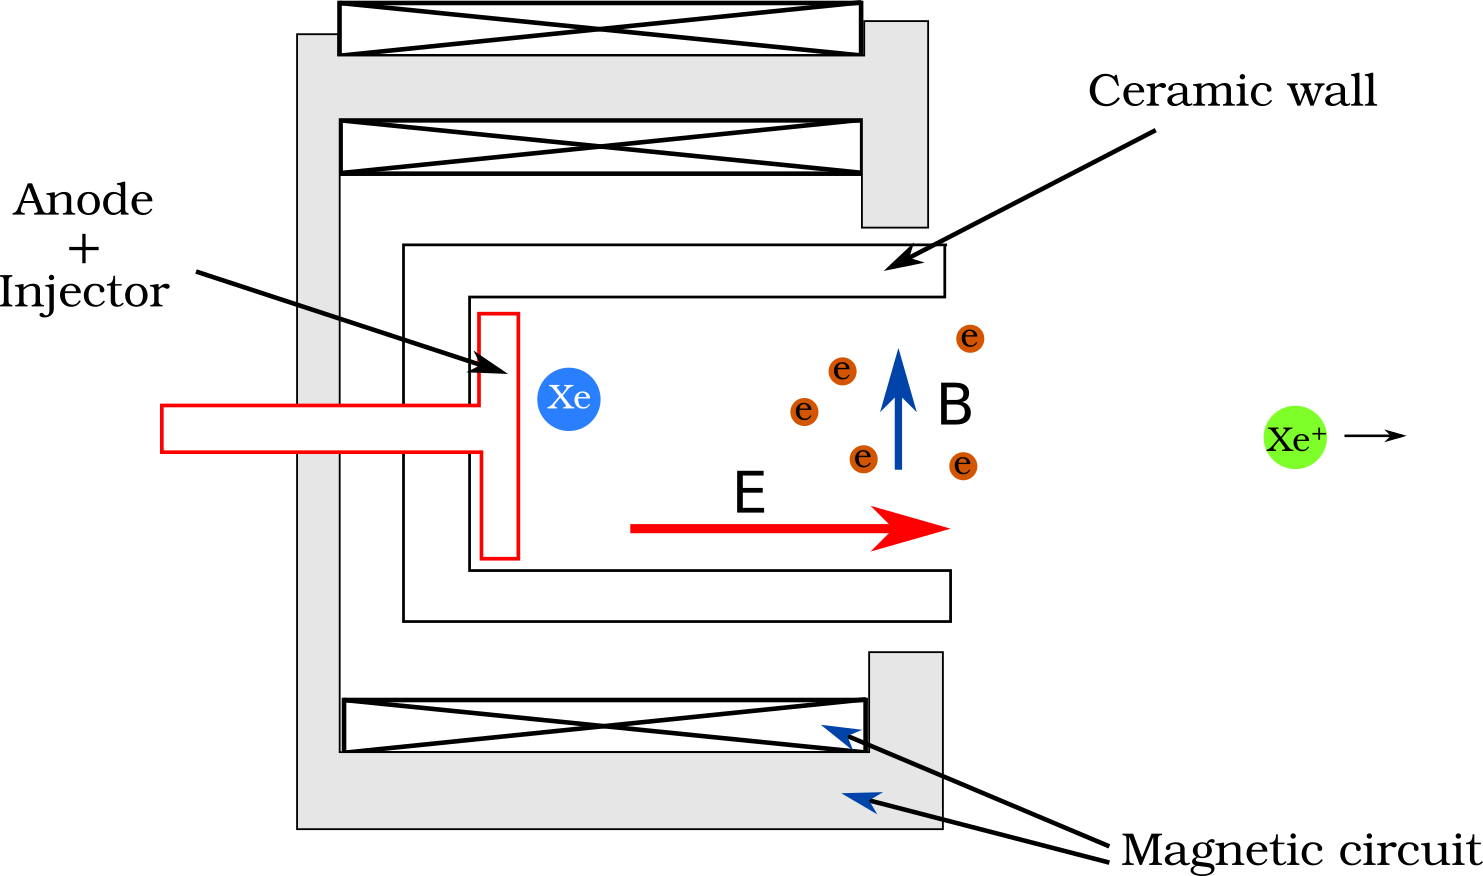
\includegraphics[scale=0.7]{images/HET.png}
		\caption{Shematic cut of an HET}
		\end{figure}
	
	\end{column}

\end{columns}	

\end{frame}

\begin{frame} 
	\frametitle{Simulation presentation} 
	\framesubtitle{ Investigating the ECDI } 
	Investigating the Electron Cyclotron Drift Instability (ECDI)
	
	\begin{columns}

	\begin{column}{0.45\linewidth}
		\begin{figure}[hbtp]
		\centering
		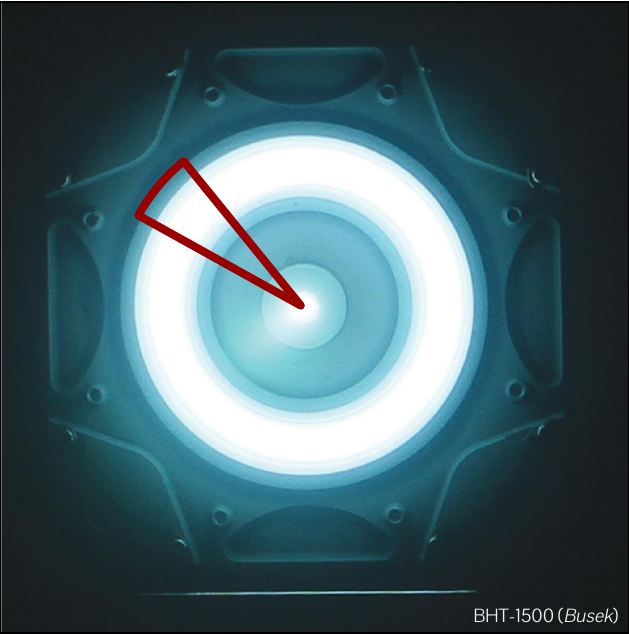
\includegraphics[scale=0.25]{images/Simulationcut.png}
	\end{figure}
	
	\end{column}

	\begin{column}{0.45\linewidth}
		\begin{figure}[hbtp]
		\centering
		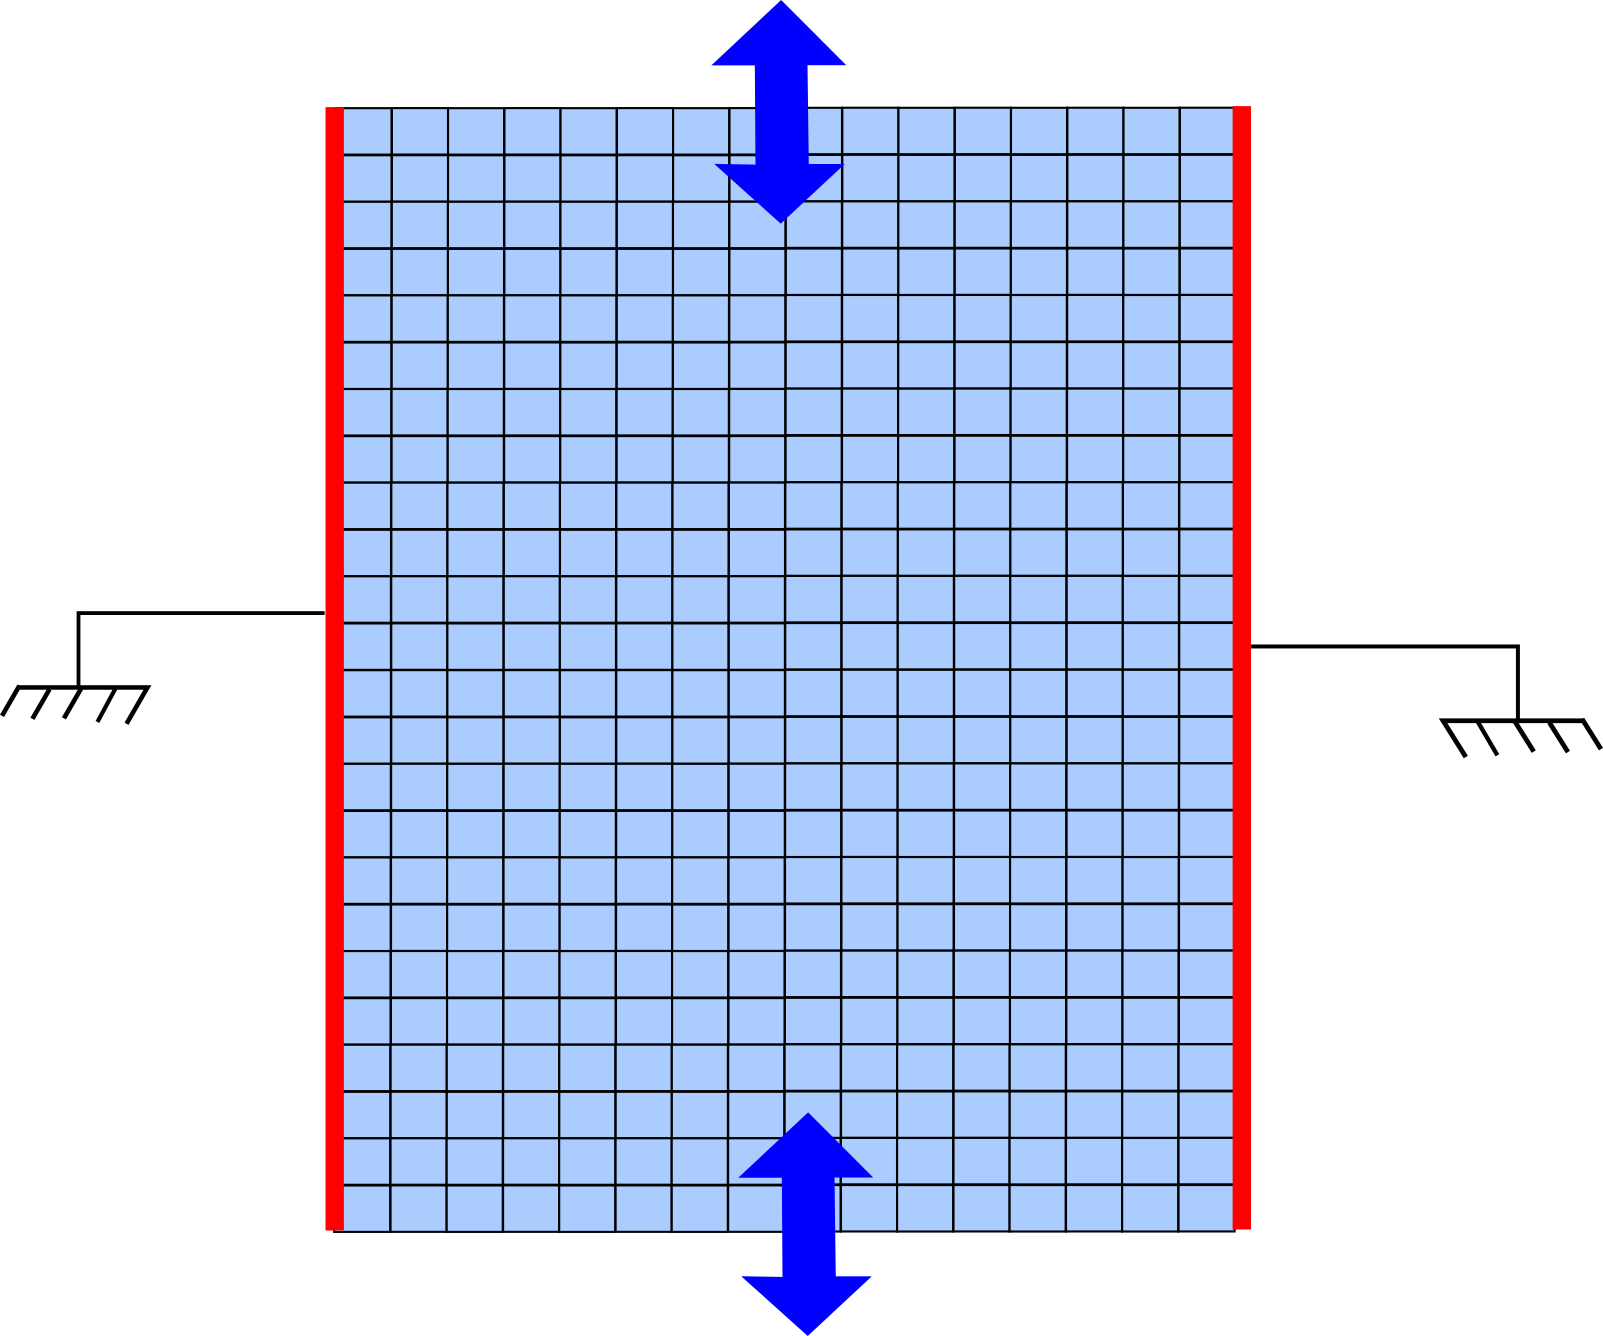
\includegraphics[scale=0.5]{images/2D_Rtheta.png}
		\caption{Shematic cut of the simulation}
		\end{figure}
	
	\end{column}


\end{columns}		
	
	
\end{frame}

\begin{frame} 
	\frametitle{Simulation results} 
	\framesubtitle{ Investigating the ECDI } 

	\begin{center}
	The Density evolution in function of time.\\
	
	\movie[width=6.65cm,height=5cm,poster,showcontrols=false]{}{images/plasma_potential_n04.mp4}
	\end{center}
\end{frame}

\begin{frame} 
	\frametitle{Simulation results} 
	\framesubtitle{ Investigating the ECDI } 
	
	\begin{columns}
	
		\begin{column}{0.45\linewidth}
			\begin{figure}[hbtp]
				\centering
				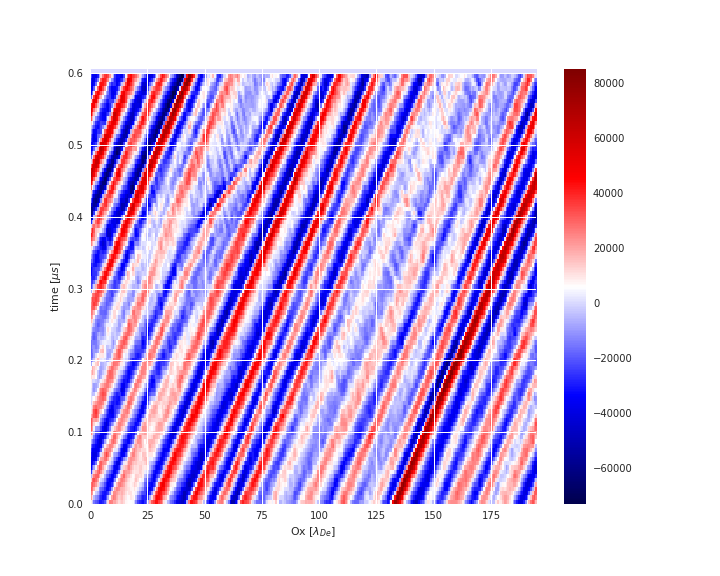
\includegraphics[scale=0.24]{images/Etheta_of_t_theta.png}
				\caption{Evolution of $E_{\theta}$ function of $t$ and $\theta$.}

			\end{figure}
		

		\end{column}	

		\begin{column}{0.45\linewidth}
			\begin{figure}[hbtp]
				\centering
				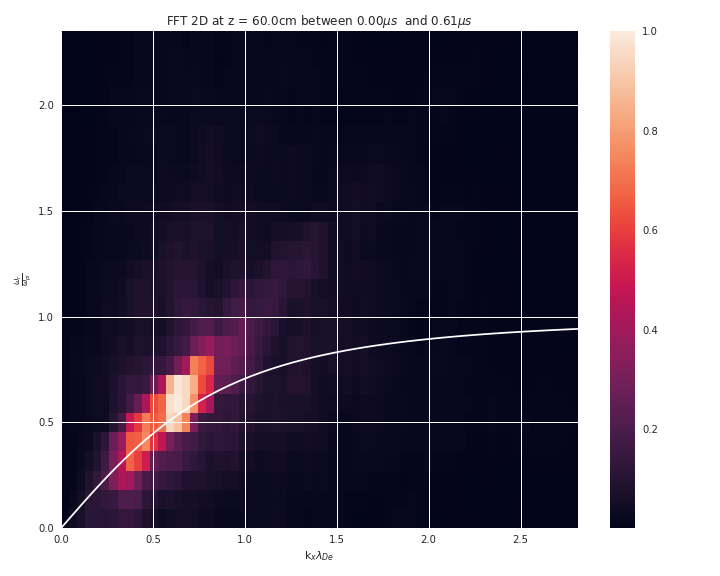
\includegraphics[scale=0.22]{images/2D_FFT.png} 
				\caption{Fourier Transform of $E_{\theta}$.}
			\end{figure}
		\end{column}	
	
	\end{columns}

\end{frame}

\begin{frame} 
\frametitle{There Is No Largest Prime Number} 
\framesubtitle{The proof uses \textit{reductio ad absurdum}.} 

\end{frame}

\begin{frame} 
\frametitle{There Is No Largest Prime Number} 
\framesubtitle{The proof uses \textit{reductio ad absurdum}.} 

\end{frame}


\begin{frame} 
\frametitle{There Is No Largest Prime Number} 
\framesubtitle{The proof uses \textit{reductio ad absurdum}.} 

\end{frame}



\begin{frame} 
\frametitle{There Is No Largest Prime Number} 
\framesubtitle{The proof uses \textit{reductio ad absurdum}.} 
\begin{theorem}
There is no largest prime number. \end{theorem} 
\begin{enumerate} 
\item<1-| alert@1> Suppose $p$ were the largest prime number. 
\item<2-> Let $q$ be the product of the first $p$ numbers. 
\item<3-> Then $q+1$ is not divisible by any of them. 
\item<1-> But $q + 1$ is greater than $1$, thus divisible by some prime
number not in the first $p$ numbers.
\end{enumerate}
\end{frame}

\begin{frame}{A longer title}
\begin{itemize}
\item one
\item two
\end{itemize}
\end{frame}

\end{document}

